%
% FH Technikum Wien
% !TEX encoding = UTF-8 Unicode
%
% Erstellung von Master- und Bachelorarbeiten an der FH Technikum Wien mit Hilfe von LaTeX und der Klasse TWBOOK
%
% Um ein eigenes Dokument zu erstellen, müssen Sie folgendes ergänzen:
% 1) Mit \documentclass[..] einstellen: Master- oder Bachelorarbeit, Studiengang und Sprache
% 2) Mit \newcommand{\FHTWCitationType}.. Zitierstandard festlegen (wird in der Regel vom Studiengang vorgegeben - bitte erfragen)
% 3) Deckblatt, Kurzfassung, etc. ausfüllen
% 4) und die Arbeit schreiben (die verwendeten Literaturquellen in Literatur.bib eintragen)
%
% Getestet mit TeXstudio mit Zeichenkodierung ISO-8859-1 (=ansinew/latin1) und MikTex unter Windows
% Zu beachten ist, dass die Kodierung der Datei mit der Kodierung des paketes inputenc zusammen passt!
% Die Kodierung der Datei twbook.cls MUSS ANSI betragen!
% Bei der Verwendung von UTF8 muss dnicht nur die Kodierung des Dokuments auf UTF8 gestellt sein, sondern auch die des BibTex-Files!
%
% Bugreports und Feedback bitte per E-Mail an latex@technikum-wien.at
%
% Versionen
% *) V0.7: 9.1.2015, RO: Modeline angepasst und verschoben
% *) V0.6: 10.10.2014, RO: Weitere Anpassung an die UK
% *) V0.5: 8.8.2014, WK: Literaturquellen überarbeitet und angepasst
% *) V0.4: 4.8.2014, WK: Initalversion in SVN eingespielt
%
\documentclass[MMR,Master,english]{twbook}
\usepackage[utf8]{inputenc}
\usepackage[T1]{fontenc}

%
% Hier biblatex & Biber konfigurieren; Vergessen Sie nicht, dass Sie biber verwenden müssen um eine Bibliothek zu erzeugen
%
\usepackage[backend=biber, style=numeric]{biblatex}
\addbibresource{Literatur.bib}

%
% Bei Bedarf bitte hier die Syntax-Highlightings anpassen
%
\usepackage[final]{listings}
\lstset{captionpos=b, numberbychapter=false,caption=\lstname,frame=single, numbers=left, stepnumber=1, numbersep=2pt, xleftmargin=15pt, framexleftmargin=15pt, numberstyle=\tiny, tabsize=3, columns=fixed, basicstyle={\fontfamily{pcr}\selectfont\footnotesize}, keywordstyle=\bfseries, commentstyle={\color[gray]{0.33}\itshape}, stringstyle=\color[gray]{0.25}, breaklines, breakatwhitespace, breakautoindent}
\lstloadlanguages{[ANSI]C, C++, [gnu]make, gnuplot, Matlab}

%Formatieren des Quellcodeverzeichnisses
\makeatletter
% Setzen der Bezeichnungen für das Quellcodeverzeichnis/Abkürzungsverzeichnis in Abhängigkeit von der eingestellten Sprache
\providecommand\listacroname{}
\@ifclasswith{twbook}{english}
{%
    \renewcommand\lstlistingname{Code}
    \renewcommand\lstlistlistingname{List of Code}
    \renewcommand\listacroname{List of Abbreviations}
}{%
    \renewcommand\lstlistingname{Quellcode}
    \renewcommand\lstlistlistingname{Quellcodeverzeichnis}
    \renewcommand\listacroname{Abkürzungsverzeichnis}
}
% Wenn die Option listof=entryprefix gewählt wurde, Definition des Entyprefixes für das Quellcodeverzeichnis. Definition des Macros listoflolentryname analog zu listoflofentryname und listoflotentryname der KOMA-Klasse
\@ifclasswith{scrbook}{listof=entryprefix}
{%
    \newcommand\listoflolentryname\lstlistingname
}{%
}
\makeatother
\newcommand{\listofcode}{\phantomsection\lstlistoflistings}

% Die nachfolgenden Pakete stellen sonst nicht benötigte Features zur Verfügung
\usepackage{blindtext}

%
% Einträge für Deckblatt, Kurzfassung, etc.
%
\title{Virtualisierung eines Echtzeit-Betriebssystems zur Steuerung eines Roboters mit Schwerpunkt auf die
Einhaltung der Echtzeit}
\author{Halil Pamuk, BSc}
\studentnumber{51842568}
%\author{Titel Vorname Name, Titel\and{}Titel Vorname Name, Titel}
%\studentnumber{XXXXXXXXXXXXXXX\and{}XXXXXXXXXXXXXXX}
\supervisor{Sebastian Rauh, MSc. BEng}
%\supervisor[Begutachter]{Titel Vorname Name, Titel}
%\supervisor[Begutachterin]{Titel Vorname Name, Titel}
%\secondsupervisor{Titel Vorname Name, Titel}
%\secondsupervisor[Begutachter]{Titel Vorname Name, Titel}
%\secondsupervisor[Begutachterinnen]{Titel Vorname Name, Titel}
\place{Wien}
\kurzfassung{Erstellung einer Echtzeit-Robotersteuerungsplattform unter Verwendung von Salamander OS, Xenomai, QEMU
und PCV-521 in der Yocto-Umgebung. Die Plattform basiert auf Salamander OS und nutzt Xenomai für Echtzeit-
Funktionen. Dazu muss im ersten Schritt die Virtualisierungsplattform evaluiert werden. (QEMU, Hyper-V, Virtual
Box, etc.) Als weiterer Schritt folgt die Anbindung eines Roboters über eine VARAN-Bus Schnittstelle. Das
gesamte System wird in der Yocto-Umgebung erstellt und konfiguriert.
Das Hauptziel der Arbeit ist es, herauszufinden, wie die Integration von Echtzeit-Funktionen und effizienten
Kommunikationssystemen in eine Robotersteuerungsplattform die Reaktionszeit und Zuverlässigkeit von
Roboteranwendungen verbessern kann}
\schlagworte{Schlagwort1, Schlagwort2, Schlagwort3, Schlagwort4}
\outline{\blindtext}
\keywords{Echtzeit, Virtualisierung, Xenomai, VARAN}
%\acknowledgements{\blindtext}

\begin{document}

\maketitle

%
% .. und hier beginnt die eigentliche Arbeit. Viel Erfolg beim Verfassen!
%
%Die folgende Gliederung von Bachelor- und Masterarbeiten ist für die Robotik-Studiengänge
%verpflichtend vorgeschrieben.
%
%- Deckblatt
%- Eidesstattliche Erklärung (digital signiert)
%- Kurzfassung und Abstract mit Schlüsselwörtern/Keywords
%- Danksagung (optional)
%- Inhaltsverzeichnis

%- Einleitung (die genannten Punkte müssen keine eigenen Unterkapitel sein, müssen aber aus der Einleitung klar hervorkommen):
%   - Stand der Technik
%   - Problem- und Aufgabenstellung
%   - Zielsetzung
%- Hauptteil -> Gliederung je nach Thema
%   - Methodik
%   - Resultate
%   - Wirtschaftliche Betrachtung (optional)
%   - Diskussion
%- Zusammenfassung und Ausblick

%- Literaturverzeichnis
%- Abbildungsverzeichnis
%- Tabellenverzeichnis
%- Abkürzungsverzeichnis (optional)
%- Glossar (optional)
%- Anhang (optional)
\chapter{Einleitung}
\blindmathpaper
\clearpage
\section{Stand der Technik}
\blindtext
\clearpage
\section{Problem- und Aufgabenstellung}
In robotics, accurate and timely control is crucial to ensure precise movements and reliable interaction with the environment. However, existing robot control systems often have limitations in terms of real-time capabilities and communication efficiency, which can have a detrimental effect on response time and reliability. The challenge is to develop a powerful real-time robot control platform that overcomes these limitations and improves the performance of robotic applications.


\clearpage
\section{Zielsetzung}

The main objective of this work is to create a real-time robot control platform that integrates Salamander OS, Xenomai, QEMU and PCV-521 in the Yocto environment. By combining these technologies, a platform is to be created that provides real-time functions and efficient communication systems. This integration is expected to lead to a significant improvement in the response time and reliability of robot applications.


%%%%%%%%%%%%%%%%%%%%%%%%%%%%%%%%%%%%%%%%%%%%%%%%%%%%%%%%%%
\clearpage
\chapter{Methodik}

The methodology of this thesis consists of several steps. First, a comprehensive literature review is conducted to understand the current trends and challenges in real-time robot control. Based on the literature study, a suitable virtualisation platform is selected. After the selection of the virtualisation platform, the robot control platform is implemented. This step includes the installation and configuration of Salamander OS, Xenomai, QEMU and PCV-521 in the Yocto environment. Once the platform has been implemented, the robot is connected via a VARAN bus interface. Finally, the platform is evaluated to determine how the integration of real-time functions and efficient communication systems improves the response time and reliability of robot applications.




- Evaluation der Virtualisierungsplattform: 
Ich werde verschiedene Virtualisierungsplattformen wie QEMU, Hyper-V, Virtual Box usw. evaluieren. Dies ist ein wichtiger Schritt, um die beste Plattform für meine Anforderungen zu finden.
  
- Erstellung und Konfiguration des Systems in der Yocto-Umgebung: 
Ich werde das Yocto-Framework verwenden, um mein Embedded Linux System zu erstellen und zu konfigurieren. Yocto bietet viele Tools und Funktionen, die mir bei der Erstellung und Konfiguration meines Systems helfen können.

- Verbesserung der Reaktionszeit und Zuverlässigkeit von Roboteranwendungen: 
Mein Hauptziel ist es, herauszufinden, wie die Integration von Echtzeitfunktionen und effizienten Kommunikationssystemen die Reaktionszeit und Zuverlässigkeit von Roboteranwendungen verbessern kann. Ich strebe an, die Leistung und Zuverlässigkeit meiner Roboteranwendungen zu verbessern, indem ich ihre Fähigkeit verbessere, in Echtzeit auf Ereignisse zu reagieren.

- Anbindung eines Roboters über eine VARAN-Bus Schnittstelle:
Ich plane, einen Roboter in mein System zu integrieren. Ich werde eine VARAN-Bus Schnittstelle verwenden, um eine schnelle und zuverlässige Kommunikation zwischen dem Roboter und dem Steuerungssystem zu gewährleisten.


\noindent Querverweise werden in \LaTeX{} automatisch erzeugt und verwaltet, damit sie leicht aktualisiert werden können. Hier wird zum Beispiel auf Abbildung \ref{Abb1} verwiesen.

\begin{figure}[!htbp]
\centering
\includegraphics[width=0.5\linewidth]{img/buchruecken}
\caption{Beispiel für die Beschriftung eines Buchrückens.}\label{Abb1}
\end{figure}
\begin{figure}[!htbp]
\centering
\includegraphics[width=0.5\linewidth]{img/buchruecken}
\caption{2. Beispiel für die Beschriftung eines Buchrückens.}\label{Abb2}
\end{figure}

Und hier ist ein Verweis auf Tabelle \ref{tab1}. Das gezeigte Tabellenformat ist nur ein Beispiel. Tabellen können individuell gestaltet werden.

\begin{table}[!htbp]
\centering
\caption{Semesterplan der Lehrveranstaltung \glqq Angewandte Mathematik\grqq.}\label{tab1}
\begin{tabular}{| p{0.3\linewidth} | p{0.3\linewidth} | p{0.3\linewidth} |}\hline
Datum & Thema & Raum\\\hline
20.08.2008 & Graphentheorie & HS 3.13\\
01.10.2008 & Biomathematik & HS 1.05\\\hline
\end{tabular}
\end{table}
\begin{table}[!htbp]
\centering
\caption{2. Semesterplan der Lehrveranstaltung \glqq Angewandte Mathematik\grqq.}\label{tab2}
\begin{tabular}{| p{0.3\linewidth} | p{0.3\linewidth} | p{0.3\linewidth} |}\hline
Datum & Thema & Raum\\\hline
20.08.2008 & Graphentheorie & HS 3.13\\
01.10.2008 & Biomathematik & HS 1.05\\\hline
\end{tabular}
\end{table}

Hier wird auf die Formel \ref{Gl1} verwiesen.

\begin{align}
x = -\frac{p}{2}\pm\sqrt{\frac{p^2}{4}-q}\label{Gl1}
\end{align}
\begin{align}
x = -\frac{p}{2}\pm\sqrt{\frac{p^2}{4}-q}\label{Gl2}
\end{align}

\begin{lstlisting}[language=C++,name={1. Beispiel},label={sc:bsp:1}]
#include <iostream>

void SayHello(void)
{
    // Kommentar
    cout << "Hello World!" << endl;
}

int main(int argc, char **argv)
{
    SayHello();
    return 0;
}
\end{lstlisting}



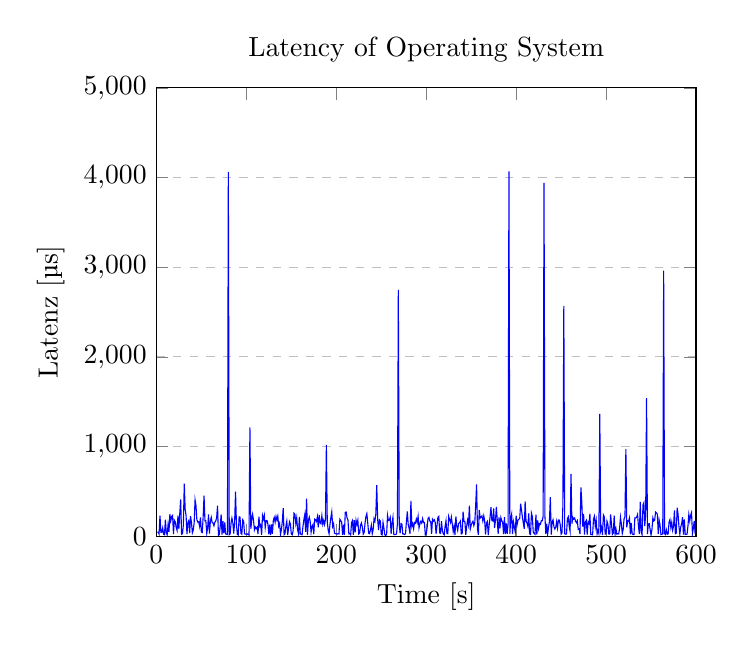
\begin{tikzpicture}
    \begin{axis}[
        title={Latency of Operating System},
        xlabel={Time [s]},
        ylabel={Latenz [µs]},
        xmin=0, xmax=600,
        ymin=0, ymax=5000,
        xtick={0,100,200,300,400,500,600},
        ytick={0,1000,2000,3000,4000,5000},
        legend pos=north west,
        ymajorgrids=true,
        grid style=dashed,
    ]
     
    \addplot[
        color=blue,
    ]
    coordinates {
        (1,46.058)(2,45.247)(3,25.008)(4,230.128)(5,44.259)(6,44.513)(7,91.711)(8,22.744)(9,16.245)(10,185.150)(11,36.711)(12,14.202)(13,130.885)(14,48.036)(15,246.716)(16,169.095)(17,219.466)(18,231.073)(19,24.619)(20,177.433)(21,160.088)(22,97.343)(23,64.062)(24,230.267)(25,78.874)(26,252.809)(27,411.265)(28,22.515)(29,27.148)(30,124.784)(31,586.676)(32,298.173)(33,230.910)(34,24.141)(35,154.979)(36,173.566)(37,33.357)(38,222.388)(39,151.711)(40,38.451)(41,67.466)(42,148.420)(43,404.945)(44,343.690)(45,184.156)(46,156.867)(47,160.473)(48,111.409)(49,209.835)(50,46.755)(51,41.262)(52,215.765)(53,453.147)(54,170.542)(55,172.430)(56,30.891)(57,94.188)(58,241.936)(59,28.899)(60,162.442)(61,210.370)(62,151.916)(63,148.249)(64,116.436)(65,156.545)(66,169.587)(67,207.000)(68,341.089)(69,9.360)(70,19.122)(71,111.249)(72,241.644)(73,16.414)(74,169.308)(75,30.421)(76,154.489)(77,25.697)(78,21.663)(79,19.417)(80,4064.225)(81,16.816)(82,24.010)(83,144.224)(84,201.855)(85,148.832)(86,30.122)(87,156.258)(88,496.579)(89,136.403)(90,19.893)(91,14.042)(92,215.474)(93,211.399)(94,30.932)(95,21.589)(96,182.871)(97,168.529)(98,26.291)(99,23.513)(100,21.540)(101,26.199)(102,15.698)(103,12.213)(104,1213.987)(105,78.669)(106,183.154)(107,242.775)(108,175.638)(109,69.769)(110,102.394)(111,83.967)(112,99.656)(113,24.573)(114,218.177)(115,108.713)(116,127.000)(117,13.701)(118,231.670)(119,190.132)(120,235.042)(121,96.299)(122,173.375)(123,175.528)(124,133.886)(125,21.396)(126,129.259)(127,12.632)(128,131.769)(129,27.551)(130,175.399)(131,208.523)(132,154.972)(133,221.602)(134,180.908)(135,223.067)(136,111.292)(137,142.352)(138,19.898)(139,74.817)(140,161.187)(141,311.376)(142,17.038)(143,27.474)(144,110.750)(145,167.509)(146,12.404)(147,90.536)(148,161.824)(149,136.528)(150,27.410)(151,15.690)(152,58.505)(153,256.667)(154,244.765)(155,140.802)(156,205.465)(157,74.799)(158,26.125)(159,215.514)(160,26.843)(161,19.168)(162,15.723)(163,111.505)(164,185.790)(165,239.944)(166,47.677)(167,418.785)(168,15.690)(169,177.398)(170,213.361)(171,162.398)(172,43.181)(173,108.263)(174,128.250)(175,23.710)(176,189.526)(177,182.737)(178,163.860)(179,217.369)(180,97.451)(181,236.625)(182,147.896)(183,138.374)(184,228.625)(185,132.462)(186,176.077)(187,130.587)(188,190.408)(189,1017.088)(190,160.770)(191,67.554)(192,27.102)(193,129.908)(194,206.303)(195,270.965)(196,109.238)(197,139.922)(198,34.335)(199,30.190)(200,24.355)(201,23.302)(202,27.776)(203,24.547)(204,188.686)(205,173.485)(206,156.228)(207,16.056)(208,128.566)(209,14.259)(210,265.675)(211,269.690)(212,203.610)(213,181.352)(214,25.724)(215,29.783)(216,15.547)(217,150.926)(218,173.356)(219,13.783)(220,178.982)(221,42.498)(222,177.951)(223,132.049)(224,177.935)(225,24.525)(226,32.250)(227,124.116)(228,147.811)(229,99.098)(230,23.038)(231,40.415)(232,145.970)(233,220.256)(234,251.117)(235,148.607)(236,33.246)(237,27.089)(238,71.276)(239,123.321)(240,26.517)(241,73.006)(242,194.473)(243,167.213)(244,249.329)(245,570.648)(246,190.634)(247,68.425)(248,180.909)(249,169.027)(250,21.083)(251,13.540)(252,152.768)(253,88.968)(254,14.848)(255,6.963)(256,23.632)(257,232.795)(258,174.460)(259,179.210)(260,210.269)(261,26.256)(262,142.122)(263,209.076)(264,17.153)(265,16.916)(266,19.901)(267,24.666)(268,139.287)(269,2746.094)(270,132.688)(271,31.390)(272,140.984)(273,134.557)(274,23.748)(275,23.969)(276,18.943)(277,27.021)(278,162.324)(279,276.631)(280,129.021)(281,87.483)(282,27.721)(283,392.561)(284,108.004)(285,140.647)(286,83.870)(287,152.610)(288,144.575)(289,192.138)(290,152.445)(291,221.906)(292,92.230)(293,139.172)(294,164.936)(295,145.246)(296,196.138)(297,152.819)(298,153.158)(299,12.769)(300,22.080)(301,92.492)(302,197.199)(303,209.789)(304,168.356)(305,163.938)(306,27.332)(307,188.547)(308,168.949)(309,183.052)(310,154.116)(311,26.958)(312,121.369)(313,211.897)(314,221.899)(315,36.295)(316,32.402)(317,166.892)(318,59.867)(319,27.105)(320,14.650)(321,110.097)(322,172.118)(323,29.988)(324,27.658)(325,220.311)(326,183.575)(327,152.368)(328,211.698)(329,134.616)(330,51.270)(331,108.671)(332,13.548)(333,219.511)(334,109.252)(335,64.613)(336,140.805)(337,149.700)(338,167.807)(339,25.758)(340,30.765)(341,273.123)(342,164.909)(343,165.589)(344,14.878)(345,112.409)(346,179.138)(347,128.386)(348,341.071)(349,80.479)(350,120.418)(351,151.436)(352,167.232)(353,117.961)(354,151.837)(355,343.459)(356,576.624)(357,83.026)(358,14.864)(359,291.525)(360,202.061)(361,214.078)(362,226.545)(363,167.546)(364,226.433)(365,171.912)(366,19.201)(367,146.997)(368,164.363)(369,13.099)(370,124.107)(371,214.734)(372,322.862)(373,173.702)(374,170.163)(375,311.086)(376,91.813)(377,176.570)(378,325.418)(379,180.390)(380,26.203)(381,210.092)(382,87.712)(383,206.417)(384,172.590)(385,155.587)(386,24.720)(387,211.070)(388,24.456)(389,141.462)(390,25.085)(391,133.946)(392,4070.018)(393,23.791)(394,196.018)(395,246.103)(396,23.463)(397,159.743)(398,105.678)(399,43.826)(400,228.944)(401,127.796)(402,177.334)(403,188.556)(404,198.069)(405,363.375)(406,286.065)(407,213.258)(408,142.917)(409,81.932)(410,387.950)(411,165.773)(412,148.521)(413,110.014)(414,254.838)(415,25.412)(416,19.918)(417,257.054)(418,218.566)(419,45.948)(420,29.893)(421,21.854)(422,240.444)(423,18.189)(424,175.604)(425,85.316)(426,140.207)(427,133.251)(428,172.613)(429,171.017)(430,220.708)(431,3939.951)(432,220.420)(433,22.360)(434,140.186)(435,20.653)(436,96.784)(437,164.221)(438,435.337)(439,17.824)(440,157.655)(441,183.606)(442,106.997)(443,79.923)(444,98.318)(445,163.483)(446,91.552)(447,180.445)(448,179.750)(449,127.103)(450,23.167)(451,37.710)(452,354.087)(453,2569.037)(454,26.980)(455,22.115)(456,24.996)(457,197.054)(458,216.713)(459,106.452)(460,53.856)(461,696.160)(462,139.231)(463,209.923)(464,191.278)(465,203.296)(466,168.068)(467,150.064)(468,173.022)(469,76.982)(470,82.013)(471,24.446)(472,544.953)(473,381.607)(474,106.719)(475,247.009)(476,16.932)(477,158.153)(478,175.496)(479,16.598)(480,155.504)(481,137.559)(482,250.553)(483,18.037)(484,17.485)(485,15.028)(486,189.511)(487,222.884)(488,105.779)(489,176.428)(490,25.272)(491,62.036)(492,27.618)(493,1364.292)(494,58.514)(495,96.686)(496,12.729)(497,238.651)(498,218.703)(499,23.869)(500,25.420)(501,167.466)(502,134.191)(503,24.254)(504,23.277)(505,242.985)(506,135.149)(507,20.173)(508,33.589)(509,228.909)(510,18.160)(511,79.284)(512,21.651)(513,28.330)(514,24.800)(515,84.395)(516,210.849)(517,133.704)(518,31.291)(519,74.501)(520,195.666)(521,215.479)(522,972.253)(523,98.867)(524,171.062)(525,165.230)(526,204.254)(527,21.464)(528,146.101)(529,27.601)(530,16.827)(531,17.296)(532,204.706)(533,202.022)(534,212.635)(535,242.466)(536,107.899)(537,24.687)(538,383.024)(539,43.742)(540,16.731)(541,348.275)(542,373.132)(543,112.767)(544,239.302)(545,1540.068)(546,23.941)(547,136.041)(548,140.292)(549,72.251)(550,13.551)(551,74.170)(552,203.932)(553,170.396)(554,178.037)(555,269.349)(556,260.202)(557,243.980)(558,24.721)(559,177.769)(560,124.189)(561,17.647)(562,21.445)(563,24.968)(564,2961.302)(565,28.545)(566,18.846)(567,71.297)(568,22.175)(569,24.419)(570,157.237)(571,185.063)(572,96.272)(573,154.349)(574,65.727)(575,112.406)(576,288.028)(577,27.610)(578,34.325)(579,317.262)(580,248.806)(581,111.234)(582,20.925)(583,103.927)(584,136.724)(585,212.379)(586,18.648)(587,186.993)(588,19.668)(589,21.342)(590,22.662)(591,110.076)(592,241.796)(593,170.161)(594,233.329)(595,263.563)(596,26.732)(597,87.702)(598,170.590)(599,26.381)
        % add all your points here
    };
    
    %\legend{Test 1}
    
    \end{axis}
    \end{tikzpicture} 

Literaturverweise sollten automatisch verwaltet werden, vor allem, wenn es viele Quellenverweise gibt. Beispiele sind  \cite{Ko05a}, \cite{Ko05b}, \cite{MiGo05}, \cite{TeGo14}, \cite{HuHa07}, \cite{HuZi10}, \cite{ZiKu07}, \cite{He07}, \cite{SIE11}, \cite{SIE14}, \cite{ISO98}, \cite{ATM11}, \cite{Hu11}, \cite{Po10}. Das verwendete Zitierformat (bzw.~das Format des Literaturverzeichnisses) ist entspechend der Vorgaben der Studiengänge zu wählen.
Es wird dringend empfohlen, BibTeX~zu verwenden (wie in diesem Beispiel).


\clearpage
\chapter{Hauptteil}
\clearpage
\chapter{Resultate}
\clearpage
\chapter{Diskussion}
\clearpage
\chapter{Zusammenfassung und Ausblick}



%
% Hier beginnen die Verzeichnisse.
%
\clearpage
\printbibliography
\clearpage

% Das Abbildungsverzeichnis
\listoffigures
\clearpage

% Das Tabellenverzeichnis
\listoftables
\clearpage

% Das Quellcodeverzeichnis
\listofcode
\clearpage

\phantomsection
\addcontentsline{toc}{chapter}{\listacroname}
\chapter*{\listacroname}
\begin{acronym}[XXXXX]
    \acro{ABC}[ABC]{Alphabet}
    \acro{WWW}[WWW]{world wide web}
    \acro{ROFL}[ROFL]{Rolling on floor laughing}
\end{acronym}

%
% Hier beginnt der Anhang.
%
\clearpage
\appendix
\chapter{Anhang A}
\clearpage
\chapter{Anhang B}
\end{document}
